\chapter{Design}

\section{Overall System Design}

\subsection{Short description of the main parts of the system}
	The system contains three main elements: The subsystem for managing meetings,
	 the subsystem for managing referral tickets and the subsystem for managing
	 resources and accounting. The meeting management subsystem will contain a
	 record of all the meetings for each member of the staff team, therefore as
	 part of the global system, there will be a representation of the staff team
	  and anyone who might be involved in any meetings. This subsystem will also
	   be responsible for the reminding the users of their meetings and informing
	    users when they've been invited to a meeting.
	The next subsystem is the system for managing support and referral tickets,
	this will automatically pass the ticket on to whoever is on the rota to deal
	with that ticket at the given time. The tickets will be listed in order of
	priority, which is set when they're submitted, the priority will increase with
	 time to ensure that nothing is ignored for too long as often the issues
	 that would be reported are very time sensitive. The tickets will be kept
	 securely in an encrypted section of the database, and each individual
	 ticket will only be accessible by people for whom it is relevant to ensure
	 confidentiality and compliance with various laws concerning such information.
	The third subsystem, designed for managing the material resources within the
	Church will consist of a record of all of the finite resources that the
	Church regularly purchases and sells, the subsystem will also keep track
	of the money throughput.
	Because many of the people who would operate this system will not be trained
	nor contractually obliged to give a satisfactory quality of service, the
	 security and access rights components of the system are of paramount
	 importance, not only to prevent breaches in confidentiality but also to
	 ensure that nobody is confused when the interface is more complicated than
	 necessary therefore the system needs to determine which parts of the system
	  are relevant to a particular person and only show them those parts.
\subsection{System flowcharts showing an overview of the complete system}

\section{User Interface Designs}
	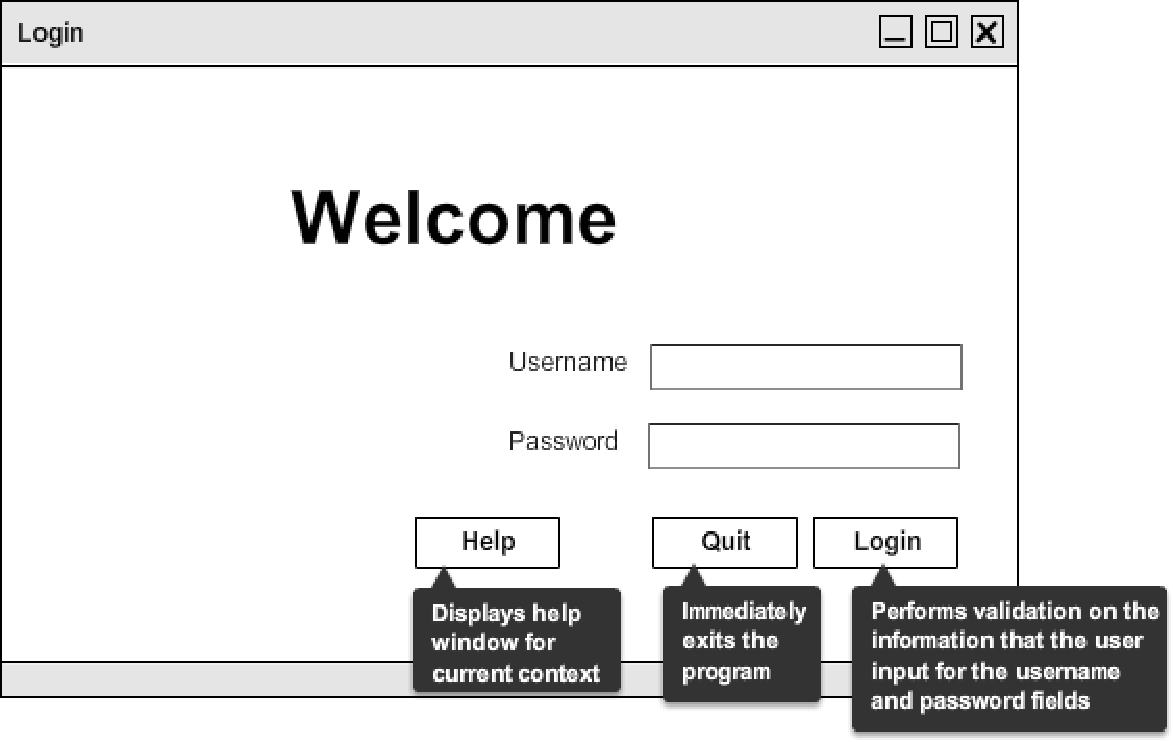
\includepdf{wireframe.pdf}
	% Put the mockflow PDF here

\section{Hardware Specification}
	The software will run on a variety of desktop Windows PCs, Windows Laptops,
	Linux/UNIX Laptops/Desktops and Apple Mac Laptops all with varying screen
	resolutions and all from different generations of hardware. The minimum
	display resolution is 1280x1024px so the GUI has to at least fit comfortably
	within this area. The software will require both a keyboard and a mouse for
	operating the UI. All of the data storage will be on either a local or a
	remote hard disk drive. The output will be displayed on a monitor.


\section{Program Structure}

\subsection{Top-down design structure charts}

% TODO: Include the diagrams from draw.io here
\begin{figure}
	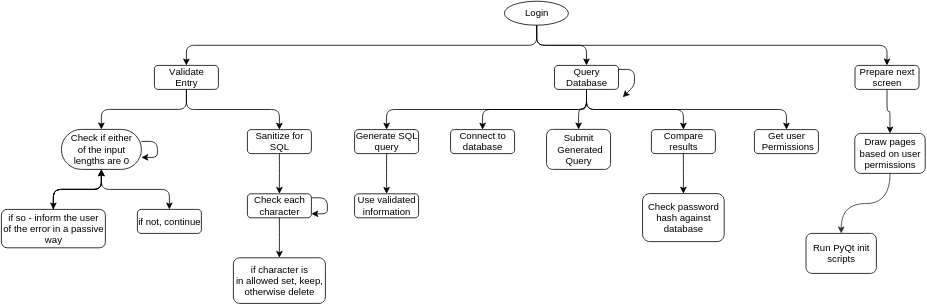
\includegraphics[width=\textwidth]{./Design/tdsl.png}
\end{figure}

\subsection{Algorithms in pseudo-code for each data transformation process}

% TODO: Use the diargams to write some pseudo-code

% TODO: Write an algorithm for the prioritized sorting feature in the tasks section

% TODO: Include the MD5 algorithm?

% TODO: Show algorithms represented by SQL?

% TODO: Show the `show different pages depending on permissions algorithm`
%		- Convert number into binary
%		- Convert binary into boolean array
%		- Go through the array and display content accordingly

% TODO:

\subsection{Object Diagrams}

% TODO: Remember to complete this in the analysis section
    \begin{figure}[H]
        \inclucegraphics[width=\textwidth]{./Design/diagrams/orld.jpg}
    \end{figure}

\subsection{Class Definitions}

% TODO: Define the software objects based on the ER diagrams.

%TODO: This in object relationship diagram
	\begin{figure}[H]
		\inlcudegraphics[width=\textwidth]{./Design/diagrams/ods.jpg}
	\end{figure}

\section{Prototyping}
	\begin{figure}[H]
		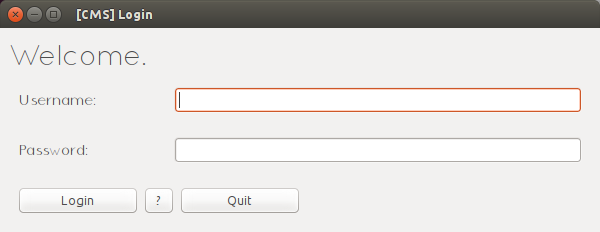
\includegraphics[width=\textwidth]{./Design/proto/1.png}
	\end{figure}
	\begin{figure}[H]
		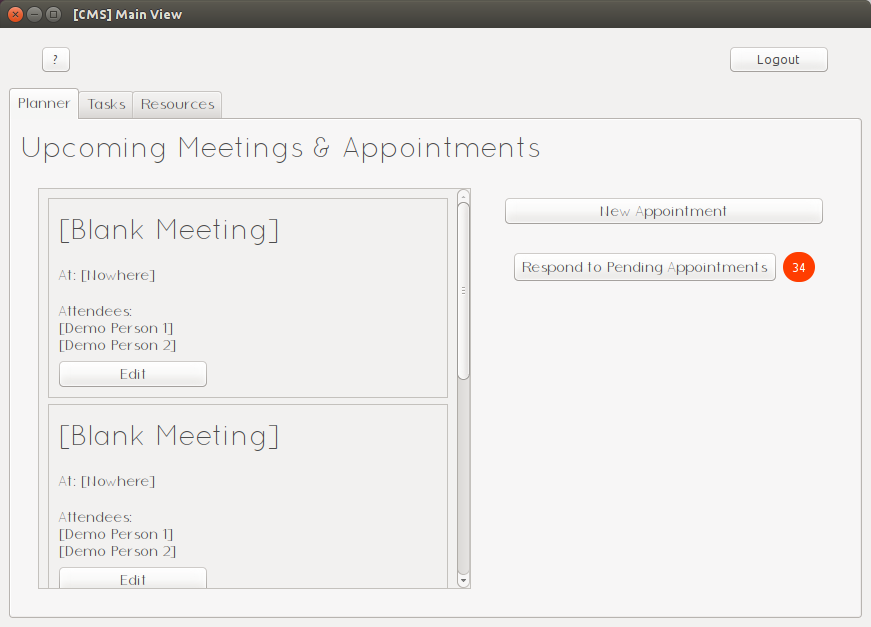
\includegraphics[width=\textwidth]{./Design/proto/2.png}
	\end{figure}
	\begin{figure}[H]
		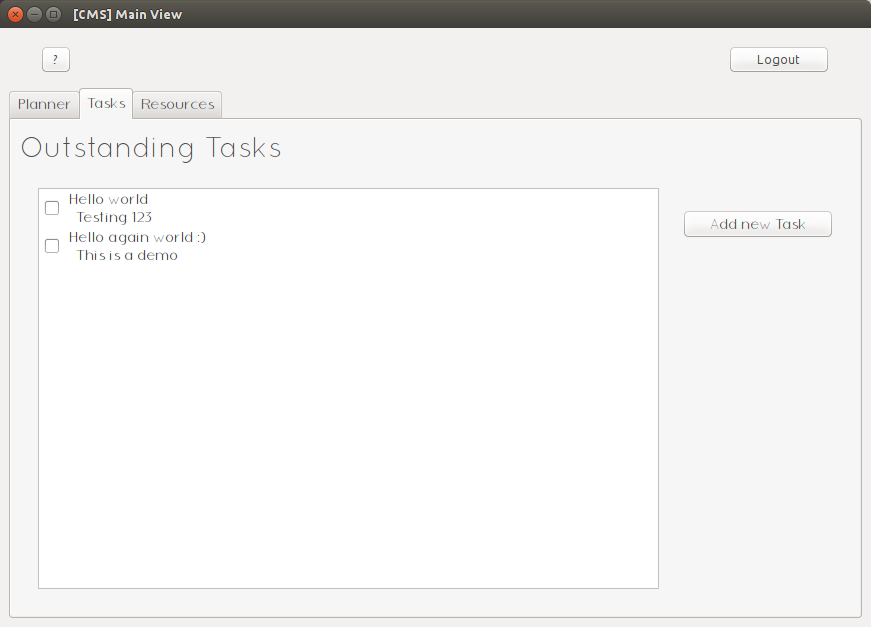
\includegraphics[width=\textwidth]{./Design/proto/3.png}
	\end{figure}
	\begin{figure}[H]
		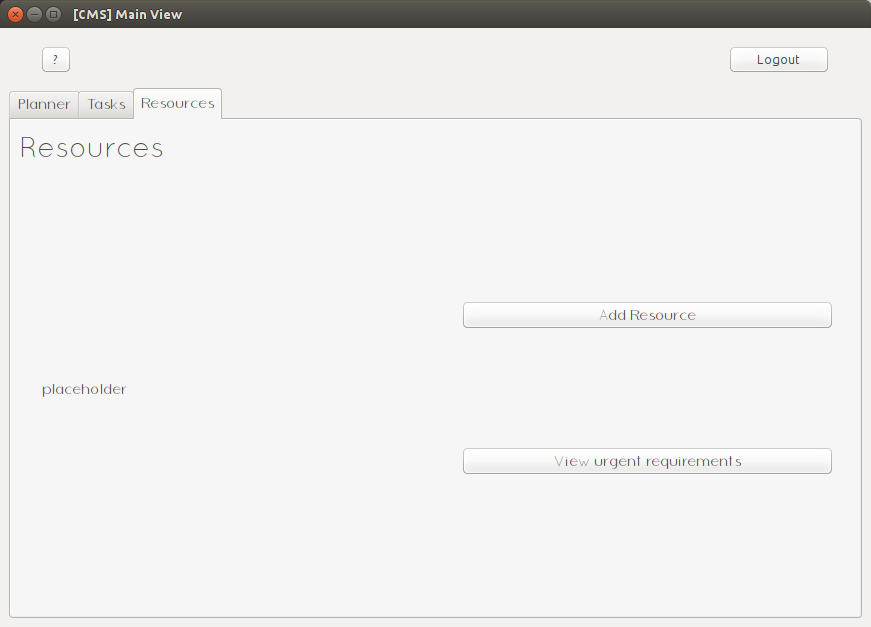
\includegraphics[width=\textwidth]{./Design/proto/4.png}
	\end{figure}
	\begin{figure}[H]
		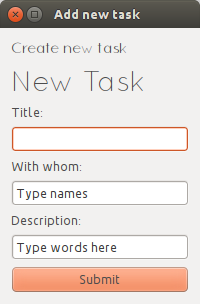
\includegraphics[width=\textwidth]{./Design/proto/5.png}
	\end{figure}
	\begin{figure}[H]
		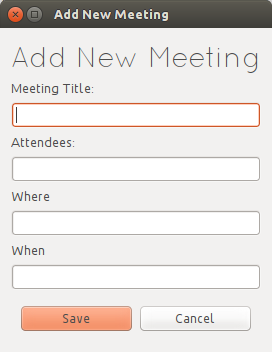
\includegraphics[width=\textwidth]{./Design/proto/6.png}
	\end{figure}
	\begin{figure}[H]
		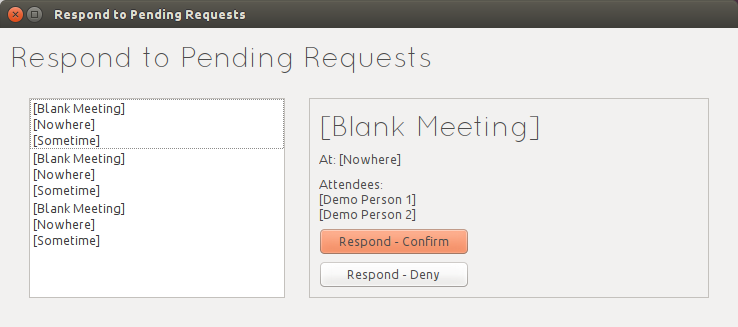
\includegraphics[width=\textwidth]{./Design/proto/7.png}
	\end{figure}
% TODO: Add screenshots from the implementation

\section{Definition of Data Requirements}

\subsection{Identification of all data input items}

\begin{itemize}
	\item Username
	\item Password
	\item User Real Name
	\item User Permissions
	\item Meetings
	\item Meeting Title
	\item Meeting Location
	\item Meeting Attendees
	\item Meeting Date & time
	\item Meeting Duration
	\item Task
	\item Task Title
	\item Task Description
	\item Task Attendees
	\item Resource
	\item Resource Name
	\item Resource Cost
	\item Resource Quantity
	\item Resource Required Quantity
\end{itemize}

\subsection{Identification of all data output items}

\begin{itemize}
	\item {All the meetings that the user owns or has confirmed their attendance
	\\which includes:
\end{itemize}
		\begin{itemize}
			\item Meeting Title
			\item Meeting Location
			\item Meeting Time & Date
			\item Meeting Duration
			\item A list of the attendees
		\end{itemize}
	}
	\item A list of all the Meetings to which the user has been invited
	\item A list of all the user's tasks.
	\item A list of the available resources, includeing their name, cost, current quantity and required quantity.
	\item An overview of the user's information.
\end{itemize}
\underline{Data output to database}
\begin{itemize}
	\item
\end{itemize}

\subsection{Explanation of how data output items are generated}

\subsection{Data Dictionary}

% TODO: Define based on Database design

\subsection{Identification of appropriate storage media}

	Because there is potential for there to be a large amount of data, which is likely to be changed and updated frequently, a single non RAID
	spinning HDD would be ample to store the data, because the system is only going to be accessed by a maximum of 10 users simultaneously, speed
	increasing RAID	is not necessary, however a redundancy drive would be useful to provide a continuous backup of the data. Solid state drives
	would not be appropriate because of the continuous reqriting of storage loactions which  would relatively quickly wear out a solid state disk
	which would not be cost effective to replace.

\section{Database Design}

\subsection{Normalisation}

\subsubsection{ER Diagrams}
	\begin{figure}[H]
		\inlcudegraphics[width=\textwidth]{./Design/diagrams/orld.jpg}
		%TODO: this needs to be redone
	\end{figure}

\subsubsection{Entity Descriptions}
User(\underline{UserID}, Username, UserFirstname, UserLastname, UserPasswordHash, Permissions)

Meeting(\underline{MeetingID}, MeetingOwner, MeetingTitle, MeetingDateTime, MeetingPlace)

MeetingAttendee(\underline{UserID}, \underline{MeetingID}, UserMeetingConfirmation)

Task(\underline{TaskID}, TaskTitle, TaskDescription, TaskOwner, TaskExpiry, Priority)

TaskAttendee(\underline{TaskID}, \underline{UserID}, Confirmed)

Resource(\underline{ResourceID}, ResourceName, ResourceCost, ResourceQuantity, ResourceRequiredQuantity)

\subsubsection{/1NF to 3NF}

	%TODO: make up some non normalised stuff then show the Normalisation process.

\subsection{SQL Queries}
	%TODO: mention output

    Database Schema:
\begin{sql}
    BEGIN TRANSACTION;
CREATE TABLE Users
                (UserID INTEGER PRIMARY KEY AUTOINCREMENT,
                Name TEXT,
                Username TEXT,
                Password TEXT,
                Permissions INTEGER
                );
CREATE TABLE Tasks
                (TaskID INTEGER PRIMARY KEY AUTOINCREMENT,
                Title TEXT,
                Description TEXT,
                Owner INTEGER,
                Attendees INTEGER
                );
CREATE TABLE TaskAttendee
                (
                TaskId INTEGER,
                UserId INTEGER
                );
CREATE TABLE `Resources` (
	`ResourceID`	INTEGER NOT NULL PRIMARY KEY AUTOINCREMENT,
	`ResourceName`	TEXT,
	`ResourceCost`	INTEGER,
	`ResourceQuantity`	INTEGER,
	`ResourceRequiredQuantity`	INTEGER
);
CREATE TABLE Meetings
                (MeetingID INTEGER PRIMARY KEY AUTOINCREMENT,
                OwnerID INTEGER,
                Title TEXT,
                ISOTime TEXT,
                Location TEXT,
                Attendees INTEGER
                );
CREATE TABLE MeetingAttendee
(
    MeetingID INTEGER,
    UserID INTEGER,
    Confirmed BOOLEAN
);


# Alright let's do this later
SELECT * FROM Users WHERE UserID = x;
SELECT UserID FROM Users WHERE (Username = \'p\');
INSERT INTO Users(Name, Username, Password, Permissions) VALUES(\'Name\', \'Username\', \'Password\', 31);
INSERT INTO Meetings(OwnerID, Title, ISOTime, Location) VALUES(x, \'Meeting Title\', \'Meeting Time\',  \'Location\');
SELECT * FROM Meetings {0};
SELECT * FROM MeetingAttendee WHERE (UserID = {0} AND Confirmed = 0);
SELECT MeetingID FROM Meetings {0};
INSERT INTO MeetingAttendee(MeetingID, UserID, Confirmed) VALUES(y, x, True);
SELECT UserID FROM MeetingAttendee WHERE (MeetingID = y)
UPDATE MeetingAttendee SET Confirmed = 1 WHERE (UserID = x AND MeetingID = y);
UPDATE MeetingAttendee SET Confirmed = 0 WHERE (UserID = x AND MeetingID = y);
DELETE FROM MeetingAttendee WHERE (UserID = x AND MeetingID = y);

SELECT * FROM Tasks {0};

SELECT TaskID FROM Tasks {0};
INSERT INTO Tasks(Title, Description, Owner, Attendees) VALUES({0});
SELECT Name FROM Users WHERE(UserID = x)

\end{sql}

\section{Security and Integrity of the System and Data}

\subsection{Security and Integrity of Data}
	The sensitive data, as defined under the data protectoin act (personal data such as dates of birth, addresses, contact details; and
	trusted information, such as referral notes or prayer requests) will be encrypted using a two-way encryption algorithm, such as the
	AES algorithm.
	The user's passwords that they use to access this sensitive data will be encrypted using a one-way hashing algorithm, such as the SHA1
	algorithm, so that if the database is accessed using a 3rd party application, the attacker will not be able to read the passwords and
	access the rest of the information using them.


\subsection{System Security}
	The system is protected by a combination of username-password authentication and a user privelleges system, where the administrator can
	change which subsystems each user has access to. Because the system uses a local database file, there is no builtin authentication for
	the data, if the system were to make use of a cloud system, such as Microsoft Azure, this problem would be avoided because of password
	protected  access to the database.

\section{Validation}

	\begin{figure}
		\begin{table}[width=\textwidth]
\centering
\begin{tabular}{llll}
\hline
\multicolumn{1}{|l|}{Item}                       & \multicolumn{1}{l|}{Example}                                          & \multicolumn{1}{l|}{Validation}                                              & \multicolumn{1}{l|}{Comments}                                                                                                                                                                                                                                                                                    \\ \hline
\multicolumn{1}{|l|}{Username}                   & \multicolumn{1}{l|}{username1}                                        & \multicolumn{1}{l|}{Presence Check, Verified against the database}           & \multicolumn{1}{l|}{The entry form immediately cancels it's verification if left empty, obviously the username is checked against the database to determine if it's a valid user.}                                                                                                                               \\ \hline
\multicolumn{1}{|l|}{Password}                   & \multicolumn{1}{l|}{Pa\$\$w0rd}                                        & \multicolumn{1}{l|}{Presence Check, checksum verified against the database.} & \multicolumn{1}{l|}{The entry form immediately cancels if this is left blank, if not left blank, the system will generate a hash of the user's input and then check that against the hash stored in the database.}                                                                                               \\ \hline
\multicolumn{1}{|l|}{Meeting Title}              & \multicolumn{1}{l|}{Dinner With the Smiths}                           & \multicolumn{1}{l|}{Presence Check}                                          & \multicolumn{1}{l|}{\begin{tabular}[c]{@{}l@{}}To ensure that a title is entered, this is how the meetings are identified for the user, so it's essential\\  that they have a name. Because often there are recurring meetings, it is not necessary to ensure that \\ the meeting title is unique.\end{tabular}} \\ \hline
\multicolumn{1}{|l|}{Meeting Attendees}          & \multicolumn{1}{l|}{username1, username2}                             & \multicolumn{1}{l|}{Validated against the database}                          & \multicolumn{1}{l|}{Usernames which are not recognised are not used when adding the MeetingAttendee database entries. The user should be informed when an invalid username is entered.}                                                                                                                          \\ \hline
\multicolumn{1}{|l|}{Meeting Location}           & \multicolumn{1}{l|}{Norwich Forum}                                    & \multicolumn{1}{l|}{Presence Check}                                          & \multicolumn{1}{l|}{The user is informed if the location field is left empty and the form will refuse to submit.}                                                                                                                                                                                                \\ \hline
\multicolumn{1}{|l|}{Meeting Start Date \& Time} & \multicolumn{1}{l|}{1/28/16 7:54PM}                                   & \multicolumn{1}{l|}{Discrete set of values}                                  & \multicolumn{1}{l|}{This will be a spin box, which is a widget that only allows the user to select input from a set list of values.}                                                                                                                                                                             \\ \hline
\multicolumn{1}{|l|}{Meeting End Date \& Time}   & \multicolumn{1}{l|}{2/21/16 3:36AM}                                   & \multicolumn{1}{l|}{Discrete set of values}                                  & \multicolumn{1}{l|}{As above but the minimum possible value will be set to the start date and time.}                                                                                                                                                                                                             \\ \hline
\multicolumn{1}{|l|}{Task Title}                 & \multicolumn{1}{l|}{File A Tax Return}                                & \multicolumn{1}{l|}{Presence Check}                                          & \multicolumn{1}{l|}{If the field is left empty when the user attempts to submit the form, the form will not submit and the user will be reminded gently that that field is required.}                                                                                                                            \\ \hline
\multicolumn{1}{|l|}{Task Attendees}             & \multicolumn{1}{l|}{username1, username2}                             & \multicolumn{1}{l|}{Validated against the database}                          & \multicolumn{1}{l|}{Usernames which are not recognised are not used when adding the TaskAttendee database entries. The user should be informed when an invalid username is entered.}                                                                                                                             \\ \hline
\multicolumn{1}{|l|}{Task Description}           & \multicolumn{1}{l|}{Make sure you fill out every single little field} & \multicolumn{1}{l|}{Presence Check}                                          & \multicolumn{1}{l|}{If the field is left empty when the user attempts to submit the form, the form will not submit and the user will be reminded gently that that field is required.}                                                                                                                            \\ \hline
\multicolumn{1}{|l|}{Resource Name}              & \multicolumn{1}{l|}{Teabags}                                          & \multicolumn{1}{l|}{Presence Check}                                          & \multicolumn{1}{l|}{If the field is left empty when the user attempts to submit the form, the form will not submit and the user will be reminded gently that that field is required.}                                                                                                                            \\ \hline
Resource Quantity                                & 100                                                                   & Presence Check, Integer Validation                                           & If the field is left empty when the user attempts to submit the form, the form will not submit and the user will be reminded gently that that field is required. The system will attempt to change the value into an integer, if it fails it will notify the user and the form will not submit.                  \\
Resource Cost                                    & £10.40                                                                & Presence check, regex check                                                  & If the field is left empty when the user attempts to submit the form, the form will not submit and the user will be reminded gently that that field is required. A regular expression will be used to check if the entered price is in a valid format (either  £\{int\}.\{int\} or \{int\}p)                     \\
Resource Required Quantity                       & 200                                                                   & Presence Check, Integer Validation                                           & If the field is left empty when the user attempts to submit the form, the form will not submit and the user will be reminded gently that that field is required. The system will attempt to change the value into an integer, if it fails it will notify the user and the form will not submit.                  \\
New Password                                     & P4\$\$w0Rd                                                             & Presence Check                                                               & If the field is left empty when the user attempts to submit the form, the form will not submit and the user will be reminded gently that that field is required.                                                                                                                                                 \\
Confirm New Password                             & P4\$\$w0Rd                                                             & Presence Check, verified against field \"New Password\"                        & If the field is left empty or does not match the field \"New Password\"  when the user attempts to submit the form, the form will not submit and the user will be reminded gently that that field is required.                                                                                                     \\
New Name                                         & Bob                                                                   & Presence Check, Regex check                                                  & If the field is left empty or contains invalid characters when scanned with a regular expression when the user attempts to submit the form, the form will not submit and the user will be reminded gently that that field is required.
\end{tabular}
\end{table}
\end{figure}

\section{Testing}

\begin{landscape}
\subsection{Outline Plan}

\begin{center}
    \begin{tabular}{|p{2cm}|p{5cm}|p{5cm}|p{4cm}|}
        \hline
        \textbf{Test Series} & \textbf{Purpose of Test Series} & \textbf{Testing Strategy} & \textbf{Strategy Rationale}\\ \hline
        Example & Example & Example & Example \\ \hline
    \end{tabular}
\end{center}

\subsection{Detailed Plan}

\begin{center}
    \begin{longtable}{|p{1.5cm}|p{2.5cm}|p{2.5cm}|p{2cm}|p{2cm}|p{2cm}|p{2cm}|p{2cm}|}
        \hline
        \textbf{Test Series} & \textbf{Purpose of Test} & \textbf{Test Description} & \textbf{Test Data} & \textbf{Test Data Type (Normal/ Erroneous/ Boundary)} & \textbf{Expected Result} & \textbf{Actual Result} & \textbf{Evidence}\\ \hline
        Example & Example & Example & Example & Example & Example & Example & Example \\ \hline
    \end{longtable}
\end{center}
\end{landscape}
